\vzmstitle{Интегрируемые биллиардны реализуют любой класс Эйлера многообразий Зейферта}
\vzmsauthor{Кибкало}{В.\,А.}
\vzmsinfo{Москва; {\it slava.kibkalo@gmail.ru}}
\vzmscaption

Рассмотрим биллиард (движение материальной точки) в плоской области (столе) с гамильтонианом $H = v_x^2 + v_y^2$ и упругим отражением от границы по закону Снелла. Пусть эта граница состоит из дуг софокусных квадрик семейства
\[ \qquad \qquad \qquad (b - \lambda) x^2 + (a - \lambda) y^2 \, = \, (a - \lambda) (b - \lambda). \qquad\qquad \,\,\, (1)\]

Такие системы интегрируемы по Лиувиллю (если внутренние углы области равны $\pi\slash 2$, а не $3\pi\slash 2$). Каждая траектория имеет каустику "--- квадрику того же семейства (1) с неким значением $0 \le \lambda \le a$ первого интеграла $\Lambda(x, y, v_x, v_y)$.

Слоение Лиувилля на фазовом пространстве таких биллиардов и их обобщений можно изучать при помощи теории топологической классификации школы А.Т. Фоменко, аналогично системам механики с двумя степенями свободы. Неособая трёхмерная поверхность постоянной энергии $Q^3_h = \{H = h \ne 0\}$ разбивается на поверхности $T_\lambda$ уровня интеграла $\Lambda = \lambda$ (на регулярные двумерные торы и конечное число особых двумерных или одномерных слоёв). Инвариант Фоменко-Цишанга "--- граф с символами перестроек в вершинах и числовыми метками "--- классифицирует такие слоения с точностью до послойной эквивалентности (подробнее см. [1]).

На основе полученных В.В.Ведюшкиной, А.Т. Фоменко и другими результатов А.Т. Фоменко сформулировал [2] гипотезу из нескольких пунктов о возможности моделировать слоения интегрируемых систем с различных точек зрения при помощи биллиардов и разных классов их обобщений (топологические биллиарды, биллиардные книжки, добавление потенциала, магнитного поля, и другие).

Некоторые пункты гипотезы уже доказаны (например, реализация любого атома [3]). В некоторых \textit{подклассах} изучаемых биллиардов были найдены топологические препятствия "--- свойство слоения, с которым оно не может быть слоением (на $Q^3_h$) биллиарда такого подкласса. Отметим: для найденных препятствий имеются такие расширенные классы биллиардов, в котором такое слоение уже реализуется.

Проверку весьма общего пункта гипотезы "--- о существовании биллиарда с произвольным инвариантом Фоменко-Цишанга "--- вполне естественно начать с моделирования <<локального>> слоения. Сформулированный А.Т. Фоменко <<локальный вариант>> гипотезы о биллиардах, в частности, ставит вопрос о возможности реализовать слоение с произвольной целочисленной меткой $n$ (тесно связанной с классом Эйлера соответствующего многообразия Зейферта, см. [1]) на произвольной <<семье>> (см. [1]) седловых атомов.

Выберем числа $b < \lambda_1 < \dots < \lambda_{k-1} < a$. В семействе (1) им отвечают гиперболы. Склеим стол $\Omega_k$ из разрезанных по ветвям этих гипербол $k$ экземпляров $\Omega_{(i)}$ стола"=эллипса. А именно, стол $\Omega_{(1)}$ разрежем по гиперболе $\lambda = \lambda_1$ на области $a_1, b_1, c_1$, стол $\Omega_{(K)}$ "--- по гиперболе $\lambda = \lambda_{k-1}$ на $a_k, b_k, c_k$, а остальные $\Omega_{(i)}$ "--- по $\lambda_{i-1}$ и $\Omega_i$ на области $a_i, x_i, b_i, y_i, c_i$.

Стол $\Omega_k$ склеим из них с перестановками $\sigma_1 = (a_2, x_2, a_1, b_1),$\, $\rho_1 = (b_1, c_1, y_2, c_2),$\, $\sigma_{k-1} = (a_{k}, b_{k}, x_{k-1}, b_{k-1}) ,$\, $\rho_{k-1} = (b_{k-1}, y_{k-1}, b_{k}, c_{k}),$\, $\sigma_i = (a_{i+1}, x_{i+1}, x_i, b_i)$ и $\rho_i = (b_{i}, y_{i}, y_{i+1}, c_{i+1})$ при $1 < i < k$.

\textbf{Теорема~1.} (Ведюшкина, К.) {\it Инвариант Фоменко-Цишанга слоения стола $\Omega_k$ изображён на рис. 2. На рёбрах $C_2 - C_2$ стоят метки $(r, \varepsilon) = (\infty, 1)$, на остальных рёбрах: $(0, 1)$.}

\textbf{Следствие~1.} Метка $n$ не препятствует моделированию слоений интегрируемых систем биллиардными книжками.

Работа выполнена при поддержке Программы Президента РФ поддержки ведущих научных школ (грант НШ-6399.2018.1, соглашение № 075-02-2018-867)




 \begin{figure}[h!]
  \center{ 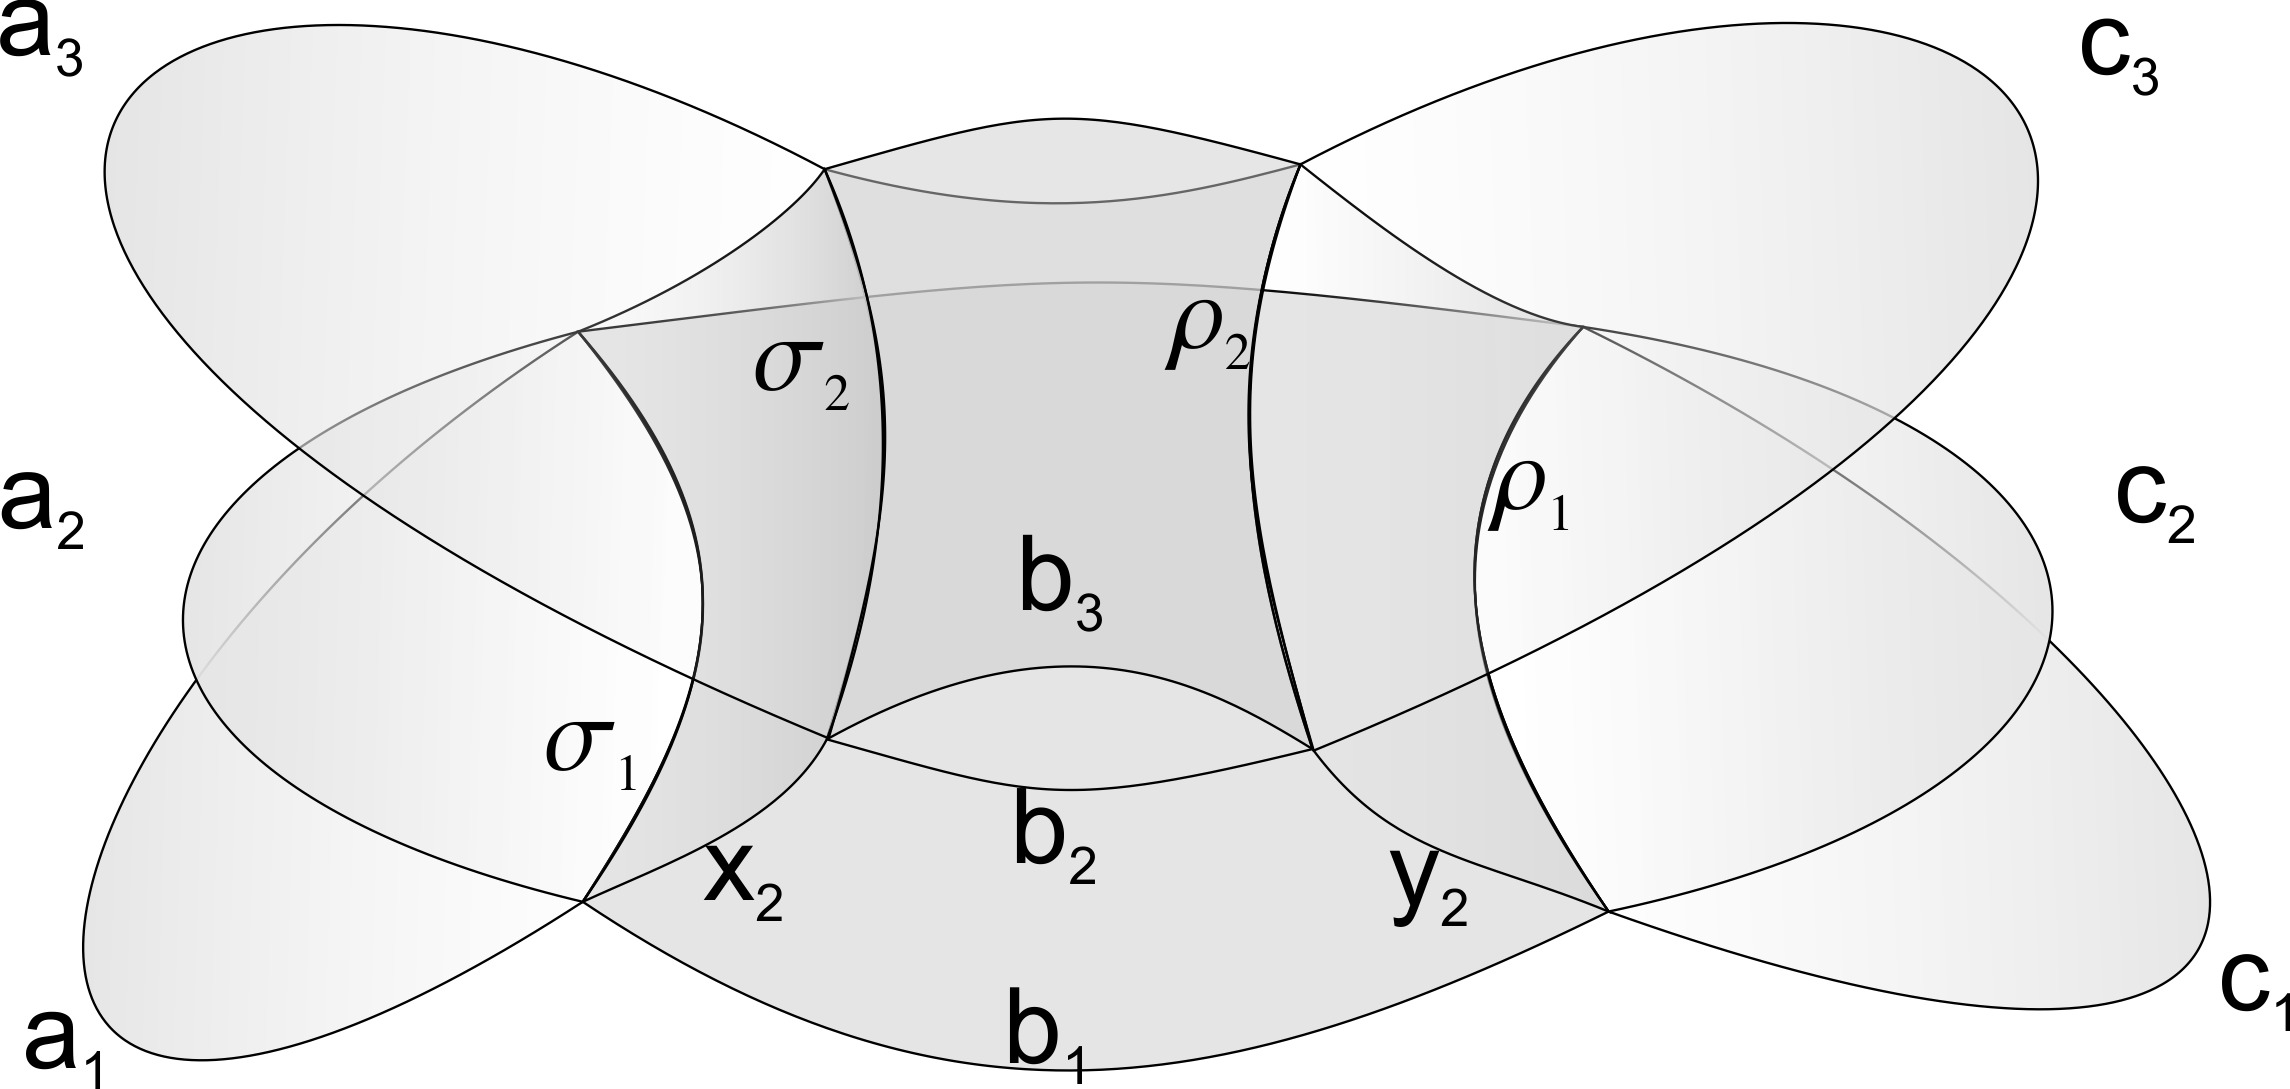
\includegraphics[width=80mm]{book.jpg}}
\caption{Биллиардная книжка $\Omega_3$ с меткой $n = 3$ на семье.} \label{WildMol}
 \end{figure}


 \begin{figure}[h!]
  \center{ 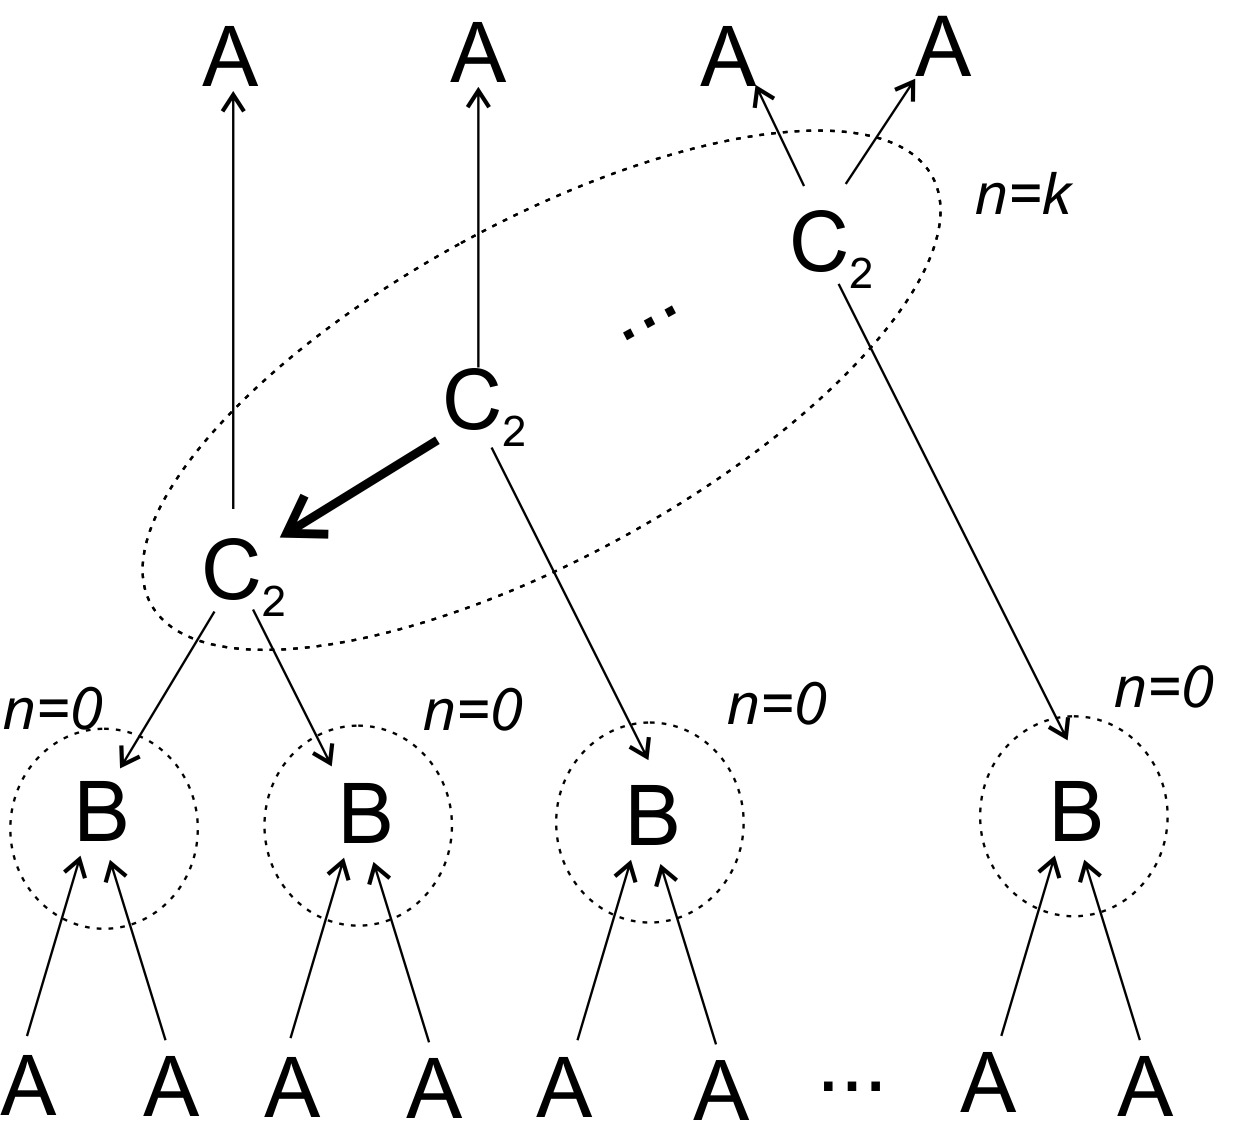
\includegraphics[width=50mm]{moleculeN.jpg}}
\caption{Метки $n$ на семьях седловых атомов для столов $\Omega_k$.} \label{WildMol}
 \end{figure}









% Оформление списка литературы
\smallskip \centerline {\bf Литература} \nopagebreak

1. {\it Болсинов В.В., Фоменко А.Т.} Интегрируемые гамильтоновы систмы: геометрия, топология, классификация. Ижевск, РХД, 1999.


2. {\it Ведюшкина В.В., Фоменко А.Т.} Бильярды и интегрируемость в геометрии и физике. Новый взгляд и новые возможности. Вестник МГУ, сер. 1, (3) 2019.

3. {\it Ведюшкина В.В., Харчева И.С.} Биллиардные книжки моделируют все трёхмерные бифуркации интегрируемых гамильтоновых систем, Матем. Сб., 209(12), 2018.

